% =====================================================================
%  Bài báo SSRC: DACL cho phân đoạn tế bào máu trong ảnh hiển vi
%  Biên dịch bằng pdfLaTeX (chạy 2 lần để cập nhật tham chiếu):
%      pdflatex Nghien_cuu_va_ung_dung_mo_hinh_DACL_cho_bai_toan_phan_doan_te_bao_mau_trong_anh_hien_vi.tex
%  figures/ : hình (Hình 1 và 3 là sơ đồ TikZ đã xuất ra PDF)
%  tables/  : bảng, mỗi bảng một file, chèn bằng \input
% =====================================================================
\documentclass{IEEEtran}
\usepackage[utf8]{vietnam}

\usepackage{cite}
\usepackage{amsmath,amssymb,amsfonts}
\usepackage{graphicx}
\usepackage{textcomp,nicefrac}
% Các gói bổ sung cho bảng và đường dẫn trong bài
\usepackage{array}
\usepackage{url}
\def\UrlBreaks{\do\/\do-}
\Urlmuskip=0mu plus 1mu
\renewcommand{\arraystretch}{1.15}
\newsavebox{\tabbox}
\def\BibTeX{{\rm B\kern-.05em{\sc i\kern-.025em b}\kern-.08em
T\kern-.1667em\lower.7ex\hbox{E}\kern-.125emX}}
\markboth{STUDENT SCIENTIFIC RESEARCH COMMUNICATION, Volume II, 2026}
{Vũ Duy Bình \MakeLowercase{\textit{và cộng sự}}: Ứng dụng mô hình DACL cho bài toán phân đoạn tế bào máu trong ảnh hiển vi}

% Ký hiệu dùng trong các công thức
\newcommand{\Lx}[1]{\mathcal{L}_{\mathrm{#1}}}
\newcommand{\KL}{\mathrm{KL}}
\newcommand{\JSD}{\mathrm{JSD}}
\newcommand{\Mix}{\mathrm{Mix}}

\begin{document}
% "Tóm tắt nội dung", "Hình", "Bảng" 
\renewcommand{\IEEEkeywordsname}{Từ khóa}
\renewcommand{\refname}{Tài liệu tham khảo}

\title{Nghiên cứu và ứng dụng mô hình ``Dual Agreement Consistency Learning'' cho bài toán phân đoạn tế bào máu trong ảnh hiển vi}
\author{Vũ Duy Bình\textsuperscript{1}, Phan Minh Khang\textsuperscript{1} và Lê Vũ Hạo\textsuperscript{1,*}
\thanks{\textsuperscript{1}Khoa Công nghệ Thông tin, Trường Đại học Công nghiệp Thành phố Hồ Chí Minh, Việt Nam (e-mail của Vũ Duy Bình: duybinh04qd@gmail.com).}
\thanks{\textsuperscript{*}Tác giả liên hệ: ThS. Lê Vũ Hạo, Khoa Công nghệ Thông tin, Trường Đại học Công nghiệp Thành phố Hồ Chí Minh.}}

\maketitle

\begin{abstract}
Tách tế bào máu khỏi nền trong ảnh hiển vi là bước cần thiết để tự động đếm và đánh giá tế bào, nhưng học sâu cần nhiều ảnh được đánh dấu thủ công. Nghiên cứu thực nghiệm này áp dụng phương pháp học bán giám sát Dual Agreement Consistency Learning (DACL), vốn được đề xuất cho ảnh siêu âm, vào ảnh hiển vi tế bào máu. Trong DACL, một mạng nhỏ và một mạng lớn cùng học từ một ít ảnh đã đánh dấu và nhiều ảnh chưa đánh dấu, đối chiếu dự đoán của nhau; sau huấn luyện, chỉ mạng nhỏ được giữ lại. Nhóm cài đặt lại DACL cùng tám phương pháp đối chứng theo giao thức chung và phân tích hàm mất mát để chọn trọng số. Trên bộ dữ liệu công khai gồm 1.328 ảnh, với 5\% hoặc 10\% ảnh được đánh dấu, mức trùng khớp với nhãn chuẩn (hệ số Dice) đạt 94,38\% và 94,46\%, cao nhất trong chín phương pháp bán giám sát. Tuy vậy, so với chính mạng nhỏ học có giám sát trên cùng số ảnh, DACL chỉ cao hơn 0,23 điểm ở mức 5\%, khác biệt không có ý nghĩa thống kê, và thấp hơn 0,14 điểm ở mức 10\%. Mỗi cấu hình chỉ được huấn luyện một lần. Mạng nhỏ có 1,58 triệu tham số, ít hơn mạng lớn khoảng 17 lần, nên phù hợp triển khai trên thiết bị phổ thông.
\end{abstract}

\begin{IEEEkeywords}
Semi-supervised learning, dual agreement, blood cell segmentation, microscopy images, UNeXt, Swin-Unet
\end{IEEEkeywords}

% ======================================================================
\section{Giới thiệu}
\label{sec:introduction}
\IEEEPARstart{Q}{uan} sát tiêu bản máu ngoại vi dưới kính hiển vi là một xét nghiệm nền tảng trong huyết học, phục vụ việc đếm tế bào và đánh giá hình thái hồng cầu, bạch cầu. Mọi phép đo định lượng như vậy đều cần xác định chính xác điểm ảnh nào thuộc tế bào và điểm ảnh nào thuộc nền, tức là bài toán phân đoạn ảnh. Khi thực hiện thủ công, công việc này tốn nhiều thời gian và phụ thuộc vào kinh nghiệm của kỹ thuật viên. Các mạng học sâu dạng mã hóa -- giải mã như U-Net~\cite{unet} đã cho phép tự động hóa bước này với độ chính xác cao trên ảnh tế bào máu~\cite{depto}.

Tuy nhiên, độ chính xác đó chỉ đạt được khi có đủ mặt nạ được gán nhãn đến từng điểm ảnh. Mỗi ảnh tiêu bản chứa hàng chục tế bào, và các tế bào chạm nhau phải được tách bằng những khe nền chỉ rộng vài điểm ảnh, khiến việc gán nhãn đòi hỏi nhiều thời gian và chuyên môn. Ngược lại, ảnh chưa gán nhãn có thể thu thập với số lượng lớn trong hoạt động xét nghiệm thường quy. Học bán giám sát khai thác sự chênh lệch này bằng cách học đồng thời từ một ít ảnh có nhãn và nhiều ảnh không nhãn~\cite{survey}. Hạn chế cố hữu của hướng tiếp cận này là mô hình có thể học theo chính dự đoán sai của nó, khiến lỗi được củng cố thay vì được sửa~\cite{confirm}.

Dual Agreement Consistency Learning (DACL)~\cite{dacl} là một khung học bán giám sát huấn luyện đồng thời một mạng tích chập nhẹ và một mạng Transformer, ràng buộc hai mạng bằng giám sát giả chéo và một hàm mất mát đồng thuận kép, và chỉ giữ lại mạng tích chập khi suy luận. Thiết kế này phù hợp với mục tiêu triển khai trên thiết bị phổ thông, nhưng khung được xây dựng cho ảnh siêu âm, nơi mỗi ảnh chứa một cấu trúc giải phẫu lớn. Ảnh hiển vi tế bào máu lại chứa nhiều đối tượng nhỏ, chạm nhau và có màu nhuộm biến thiên. Theo hiểu biết của nhóm tác giả, chưa có nghiên cứu đánh giá DACL trên loại ảnh này trong cùng điều kiện với các phương pháp bán giám sát khác, và cách các thành phần mất mát tương tác với nhau khi mỗi vòng lặp chỉ có rất ít ảnh có nhãn cũng chưa được phân tích.

Mục tiêu của nghiên cứu là xây dựng một mô hình phân đoạn tế bào máu dựa trên khung DACL, đạt độ chính xác cao khi chỉ 5\% hoặc 10\% ảnh huấn luyện được gán nhãn và chỉ dùng mạng tích chập nhẹ khi suy luận. Nghiên cứu đặt ra ba câu hỏi: (1) mô hình đạt độ chính xác như thế nào so với tám phương pháp bán giám sát tiêu biểu và so với học có giám sát trên cùng số nhãn; (2) lợi ích của mô hình thể hiện ở loại lỗi nào và tập trung ở những ảnh nào; (3) các thành phần mất mát tương tác ra sao và cần chọn trọng số thế nào để huấn luyện ổn định. Mọi phương pháp được cài đặt lại với cùng cách chia dữ liệu, tiền xử lý và lịch huấn luyện nhằm hạn chế khác biệt do điều kiện thí nghiệm, dù chúng vẫn khác nhau về số mạng, cách khởi tạo và trọng số mặc định (Mục~\ref{sec:baselines}). Phạm vi nghiên cứu giới hạn ở bài toán phân đoạn ngữ nghĩa hai lớp tế bào -- nền trên một bộ dữ liệu công khai.

Nghiên cứu được định vị là một nghiên cứu thực nghiệm và phân tích ứng dụng, không đề xuất kiến trúc hay hàm mất mát mới. Kiến trúc ba mạng cùng các thành phần giám sát giả chéo, nhất quán nội suy và đồng thuận kép được kế thừa nguyên vẹn từ DACL~\cite{dacl}. Phần việc của nhóm tác giả gồm: (1) chuyển DACL từ ảnh siêu âm sang ảnh hiển vi tế bào máu, tái triển khai DACL cùng tám phương pháp đối chứng trong một giao thức thống nhất, có mã nguồn để tái lập; (2) phân tích số hạng entropy của hàm đồng thuận kép thông qua độ phân kỳ Jensen -- Shannon, và dùng kết quả này cùng độ lớn các thành phần mất mát để lựa chọn trọng số; (3) đánh giá bằng kiểm định thống kê trên từng ảnh kiểm thử, phân tích sai số theo loại lỗi, độ khó và mật độ tế bào, kèm kiểm tra ảnh trùng lặp giữa các tập. Điều mới của nghiên cứu nằm ở bằng chứng thực nghiệm về hành vi của DACL trên miền ảnh hiển vi và ở phân tích cơ chế của hàm mất mát; phạm vi các kết luận giới hạn ở một bộ dữ liệu, hai mức nhãn và một lần huấn luyện cho mỗi cấu hình. Phần còn lại của bài báo được tổ chức như sau: Phần~\ref{sec:method} trình bày mô hình và phương pháp, Phần~\ref{sec:results} trình bày thực nghiệm, kết quả và thảo luận, và Phần~\ref{sec:conclusion} là kết luận.

% ======================================================================
\section{Mô hình và phương pháp}
\label{sec:method}

\subsection{Thiết kế nghiên cứu}

Thiết kế nghiên cứu nhằm hạn chế khác biệt về điều kiện thí nghiệm giữa các phương pháp. Nghiên cứu áp dụng phương pháp thực nghiệm có đối chứng, trong đó biến độc lập là phương pháp huấn luyện và biến phụ thuộc là các độ đo chất lượng phân đoạn trên từng ảnh kiểm thử. Quy trình gồm năm giai đoạn như Hình~\ref{fig:flow}: thu thập dữ liệu, tiền xử lý và phân chia, xây dựng mô hình, huấn luyện và đánh giá. Mười một mô hình, gồm UNeXt và Swin-Unet học có giám sát, tám phương pháp bán giám sát đối chứng và DACL, đã được huấn luyện với cùng cách chia dữ liệu, cùng tiền xử lý, cùng bộ tối ưu và cùng số vòng lặp. Những yếu tố chưa được đồng nhất hoàn toàn, gồm cách khởi tạo, số mạng và trọng số của từng phương pháp, được nêu ở Mục~\ref{sec:baselines}.

\begin{figure*}[!t]
\centering
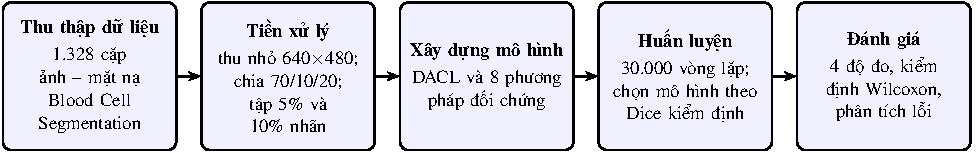
\includegraphics{figures/fig_flow.pdf}
\caption{Quy trình nghiên cứu.}
\label{fig:flow}
\end{figure*}

\subsection{Dữ liệu nghiên cứu}

Nghiên cứu sử dụng bộ dữ liệu công khai Blood Cell Segmentation do Depto và cộng sự công bố~\cite{depto}, phân phối theo giấy phép MIT~\cite{repo}. Bộ dữ liệu gồm 1.328 ảnh hiển vi tiêu bản máu và 1.328 mặt nạ nhị phân tế bào/nền, không kèm thông tin về người bệnh. Trong đó, 1.208 ảnh có kích thước 1600$\times$1200 và 120 ảnh có kích thước 1944$\times$1383 điểm ảnh. Ở độ phân giải 640$\times$480, điểm ảnh tế bào chiếm trung bình 29,4\% diện tích ảnh (từ 4,2\% đến 73,2\%), và mỗi mặt nạ có trung bình 58,5 vùng liên thông (trung vị 56).

\begin{figure*}[!t]
\centering
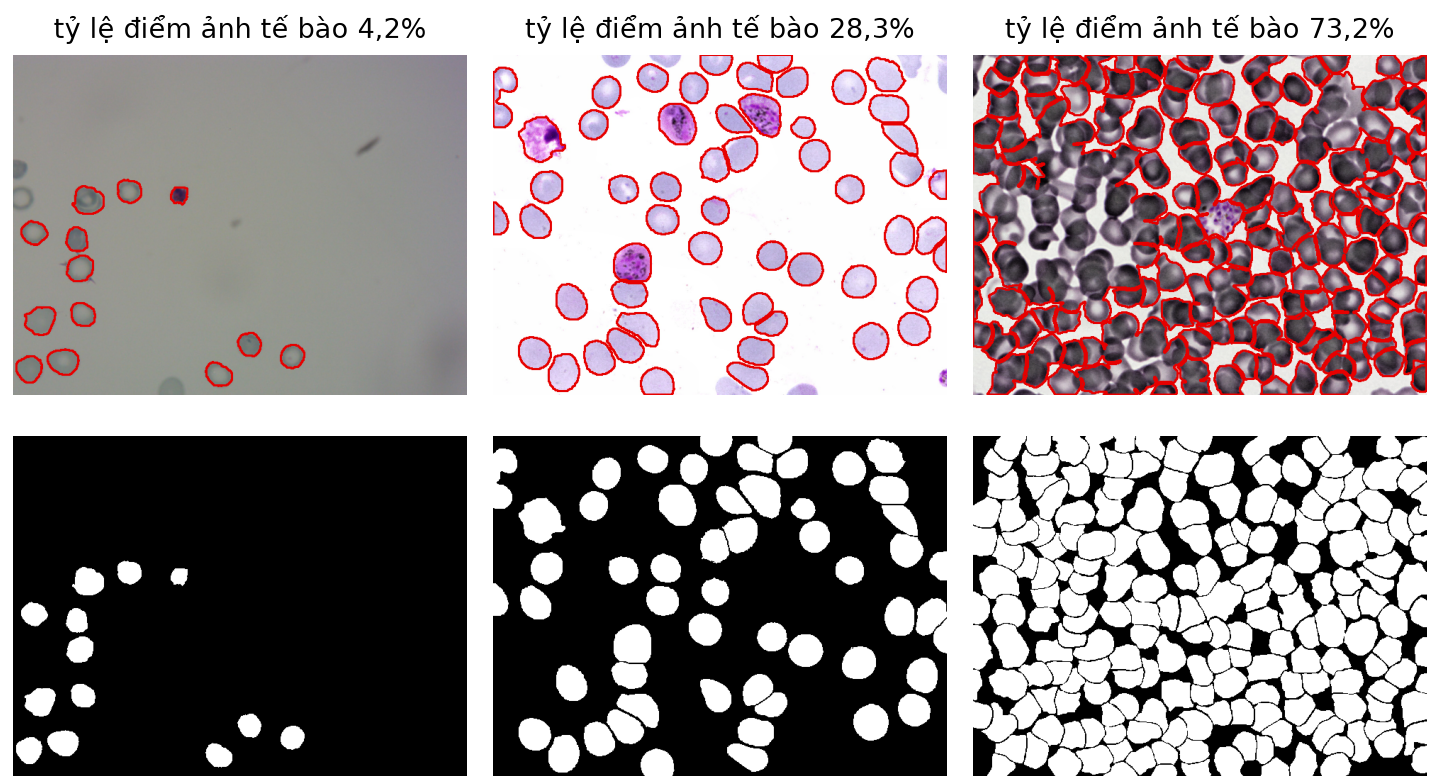
\includegraphics[width=0.78\textwidth]{figures/dataset_examples.png}
\caption{Ba ảnh có tỷ lệ điểm ảnh tế bào thấp nhất, trung vị và cao nhất (hàng trên: ảnh và đường viền mặt nạ; hàng dưới: mặt nạ).}
\label{fig:data}
\end{figure*}

Hình~\ref{fig:data} cho thấy ba đặc điểm gây khó cho bài toán. Thứ nhất, màu nền và màu nhuộm khác nhau rõ rệt giữa các ảnh, từ nền xám lục với tế bào nhạt màu đến nền trắng với tế bào tím. Thứ hai, mọi loại tế bào, kể cả tế bào có vùng bắt màu tím đậm, được gán cùng một lớp. Thứ ba, ở ảnh có mật độ cao, các tế bào chạm nhau được tách bằng những khe nền chỉ rộng vài điểm ảnh, vốn dễ bị mất khi thu nhỏ ảnh.

Ảnh đã được thu nhỏ về 640$\times$480 (nội suy theo diện tích cho ảnh, láng giềng gần nhất cho mặt nạ), mặt nạ được nhị phân hóa với ngưỡng 127, rồi dữ liệu được chia ngẫu nhiên với hạt giống 2026 theo tỷ lệ 70/10/20 (Bảng~\ref{tab:split}). Các tập có nhãn 5\% và 10\% được lấy từ đầu danh sách huấn luyện đã xáo trộn; phần còn lại được dùng như ảnh không nhãn, và mặt nạ của chúng không được đọc khi huấn luyện. Khi đưa vào mạng, ảnh được thu nhỏ về 224$\times$224 và chuẩn hóa theo thống kê ImageNet. Ảnh có nhãn được tăng cường trực tuyến bằng các phép hình học (lật, xoay 90\textdegree, affine, biến dạng đàn hồi), phép màu (color jitter, biến thiên nhuộm HED~\cite{hed}, gamma, CLAHE) và phép suy giảm chất lượng (làm mờ, nhiễu Gauss), nhằm mô phỏng sự khác biệt về nhuộm và điều kiện chụp giữa các tiêu bản.

\begin{table}[!t]
\caption{Phân chia tập dữ liệu}
\label{tab:split}
\centering
\setlength{\tabcolsep}{3pt}
\begin{tabular}{|p{100pt}|c|c|c|}
\hline
Tập dữ liệu & Số ảnh & 5\% nhãn & 10\% nhãn \\
\hline
Huấn luyện (có nhãn / không nhãn) & 930 & 46 / 884 & 93 / 837 \\
Kiểm định & 133 & 133 & 133 \\
Kiểm thử & 265 & 265 & 265 \\
\hline
\end{tabular}
\end{table}


Hai tập con có nhãn lồng nhau, tức tập 5\% nằm trọn trong tập 10\%, nên khác biệt giữa hai mức nhãn chỉ đến từ 47 ảnh có nhãn bổ sung. Tập kiểm định và tập kiểm thử giống nhau ở mọi mức nhãn và ở mọi phương pháp.

Để kiểm tra tính độc lập giữa các tập, toàn bộ 1.328 ảnh đã được so sánh theo ba cách: mã băm MD5 của tệp gốc, mã băm của dữ liệu điểm ảnh sau khi thu nhỏ về 640$\times$480, và hai mã băm cảm nhận 64 bit (pHash, dHash) kèm hệ số tương quan chuẩn hóa trên ảnh xám 64$\times$48. Không có tệp hay ảnh nào trùng khít. Trong 405.385 cặp ảnh thuộc hai tập khác nhau, chỉ một cặp gần trùng được phát hiện, gồm một ảnh không nhãn của tập huấn luyện và một ảnh kiểm thử, với hệ số tương quan 0,999 và khoảng cách pHash bằng 0; kiểm tra trực quan cho thấy đây là cùng một trường quan sát được chụp với độ sáng hơi khác nhau. Cặp gần nhất tiếp theo chỉ có hệ số tương quan 0,41. Loại ảnh kiểm thử này ra làm Dice trung bình của DACL, UNeXt học có giám sát, PCPCS và DSTCT thay đổi không quá 0,01 điểm, nên các kết quả vẫn được báo cáo trên đủ 265 ảnh. Các phép so sánh toàn ảnh này không phát hiện được những trường quan sát chồng lấn một phần, và bộ dữ liệu không cung cấp mã tiêu bản hay mã người bệnh. Vì vậy, nghiên cứu chưa thể bảo đảm tính độc lập ở cấp tiêu bản; điều này không có nghĩa là đã có rò rỉ dữ liệu, nhưng giới hạn khả năng khái quát của kết quả sang tiêu bản mới.

\subsection{Mô hình DACL}
\label{sec:dacl}

Mô hình nhằm tận dụng một Transformer dung lượng lớn khi huấn luyện để nâng chất lượng của một mạng tích chập nhẹ dùng khi triển khai. Kiến trúc ba mạng và các hàm mất mát trình bày trong mục này được giữ nguyên theo khung DACL~\cite{dacl}, như minh họa trong Hình~\ref{fig:dacl}; nhóm tác giả tái triển khai chúng và chỉ xác định thêm các chi tiết cài đặt mà khung gốc không nêu, như hệ số EMA của mạng giáo viên. Mạng tích chập $f^1$ là UNeXt~\cite{unext} với số kênh nhánh mã hóa \{32, 64, 128, 160, 256\}, gồm 1,58 triệu tham số và 1,80 GFLOPs ở đầu vào 224$\times$224; đây là mạng duy nhất được dùng khi suy luận. Mạng Transformer $f^2$ là Swin-Unet~\cite{swinunet} dựa trên Swin Transformer~\cite{swin}, phiên bản tiny với cửa sổ 7$\times$7, gồm 27,17 triệu tham số và 12,15 GFLOPs, được khởi tạo từ trọng số tiền huấn luyện trên ImageNet~\cite{imagenet}. Mạng giáo viên $f^{\mathrm{ema}}$ có cùng kiến trúc với Swin-Unet; tham số của nó được cập nhật bằng trung bình trượt hàm mũ (EMA) với hệ số 0,99, giá trị do nhóm chọn theo các phương pháp đối chứng vì khung gốc không nêu, và mạng được nhóm đặt ở chế độ suy luận để mục tiêu sinh ra không bị ảnh hưởng bởi stochastic depth.

\begin{figure}[!t]
\centering
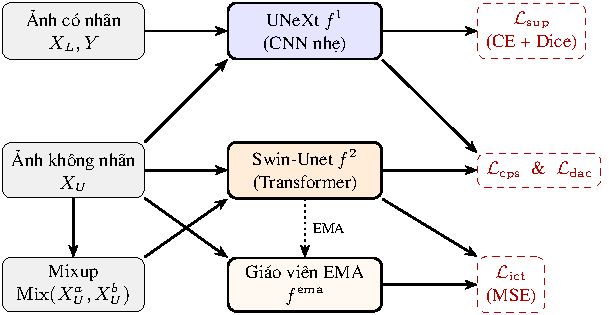
\includegraphics[width=\columnwidth]{figures/fig_dacl.pdf}
\caption{Sơ đồ tổng quát của mô hình DACL.}
\label{fig:dacl}
\end{figure}

Ở mỗi vòng lặp, một lô gồm một ảnh có nhãn và bốn ảnh không nhãn được đưa vào mô hình. Ảnh có nhãn giám sát trực tiếp cả hai mạng học sinh. Ảnh không nhãn tham gia ba ràng buộc: giám sát giả chéo giữa UNeXt và Swin-Unet, nhất quán nội suy giữa Swin-Unet và giáo viên, và đồng thuận kép giữa hai mạng học sinh. Các mục dưới đây trình bày lại từng hàm mất mát của DACL theo một hệ ký hiệu thống nhất, kèm diễn giải của nhóm tác giả về vai trò của chúng.

\subsubsection{Mất mát có giám sát}

Các mục dưới đây dùng chung một hệ ký hiệu. Với ảnh đầu vào $x$, mạng thứ $i$ ($i=1$ cho UNeXt, $i=2$ cho Swin-Unet) cho ra bản đồ logit $f^i(x)$ và bản đồ xác suất $p^i=\mathrm{softmax}(f^i(x))$, trong đó $p^i_c(u)$ là xác suất điểm ảnh $u$ thuộc lớp $c$. Bài toán có $C=2$ lớp (nền và tế bào), $\Omega$ là tập điểm ảnh của ảnh và $|\Omega|=H\times W$ là số điểm ảnh.

Với ảnh có nhãn $X_L$ và mặt nạ $Y$ biểu diễn dưới dạng one-hot $y_c(u)$, mỗi mạng được huấn luyện bằng tổng của entropy chéo $H$ và mất mát Dice $D$, theo cùng dạng hàm được dùng trong khung DACL~\cite{dacl}:
\begin{gather}
  \Lx{sup}^{i} = H(p^i, Y) + D(p^i, Y), \quad i\in\{1,2\}, \label{eq:sup}\\
  H(p, Y) = -\frac{1}{|\Omega|}\sum_{u\in\Omega}\sum_{c} y_c(u)\log p_c(u), \label{eq:ce}\\
  D(p, Y) = 1-\frac{1}{C}\sum_{c}\frac{2\sum_{u} p_c(u)\,y_c(u)+\varepsilon}{\sum_{u} p_c(u)+\sum_{u} y_c(u)+\varepsilon}. \label{eq:dice}
\end{gather}
Entropy chéo phạt từng điểm ảnh một cách độc lập: điểm ảnh nào bị gán xác suất thấp cho lớp đúng sẽ đóng góp mất mát lớn, nên thành phần này cho gradient ổn định ngay từ đầu huấn luyện. Do mọi điểm ảnh có trọng số như nhau, lớp chiếm nhiều diện tích sẽ chi phối giá trị mất mát; với tỷ lệ điểm ảnh tế bào trung bình 29,4\%, lớp nền chiếm ưu thế. Mất mát Dice~\cite{dice} khắc phục điểm này bằng cách đo độ trùng khớp ở cấp vùng cho từng lớp rồi lấy trung bình, nên lớp tế bào được đối xử ngang với lớp nền bất kể diện tích. Trong mỗi phân số, tử số đo phần giao giữa dự đoán và nhãn, mẫu số đo tổng diện tích của hai vùng, còn hằng số $\varepsilon=10^{-5}$ tránh chia cho 0; các tổng được tính trên toàn bộ ảnh trong lô. Hai mạng đều được giám sát bằng ảnh có nhãn, nên phần có giám sát của mô hình là $\Lx{sup}^{1}+\Lx{sup}^{2}$.

\subsubsection{Giám sát giả chéo}

Thành phần này khai thác ảnh không nhãn bằng cách để hai mạng dạy lẫn nhau, theo ý tưởng của Deep Co-Training~\cite{dct} và Cross Pseudo Supervision~\cite{cps} mà khung DACL kế thừa~\cite{dacl}. Với ảnh không nhãn $X_U$, mỗi mạng sinh nhãn giả one-hot bằng cách chọn lớp có xác suất lớn nhất tại từng điểm ảnh:
\begin{equation}
  \tilde{Y}^{i}(u) = \mathrm{onehot}\Big(\operatorname*{arg\,max}_{c}\; p^{i}_{c}(u)\Big). \label{eq:pseudo}
\end{equation}
Nhãn giả của mạng này được dùng làm mục tiêu cho mạng kia, với đúng dạng hàm của mất mát có giám sát:
\begin{multline}
  \Lx{cps} = \big[H(p^1,\tilde{Y}^2)+D(p^1,\tilde{Y}^2)\big] \\
  + \big[H(p^2,\tilde{Y}^1)+D(p^2,\tilde{Y}^1)\big]. \label{eq:cps}
\end{multline}
Gradient không được lan truyền qua nhãn giả: $\tilde{Y}^2$ được coi là hằng số khi cập nhật UNeXt, và $\tilde{Y}^1$ được coi là hằng số khi cập nhật Swin-Unet. Nếu cho gradient đi qua, cách đơn giản nhất để giảm mất mát là làm hai mạng cùng thay đổi dự đoán về phía nhau mà không cần dự đoán đúng hơn. Việc dùng nhãn giả của mạng kia thay vì của chính mình giúp giảm thiên lệch xác nhận. Một mạng tự huấn luyện trên nhãn giả của nó sẽ củng cố chính lỗi của nó, trong khi hai mạng có kiến trúc khác nhau thường mắc lỗi ở những vị trí khác nhau~\cite{ctct}. UNeXt thiên về đặc trưng cục bộ của tích chập, còn Swin-Unet nắm bắt quan hệ ở khoảng cách xa nhờ cơ chế tự chú ý, nên chỗ sai của mạng này có cơ hội được mạng kia sửa. Theo Wang và cộng sự~\cite{dacl}, nhãn giả được xử lý bằng cả entropy chéo và Dice như nhãn thật. Điều này làm $\Lx{cps}$ có độ lớn cùng bậc với $\Lx{sup}$, và là lý do trọng số $\lambda$ cần được xem xét cẩn thận ở Mục~\ref{sec:weights}.

\subsubsection{Nhất quán nội suy}

Thành phần thứ hai áp dụng nguyên lý của Interpolation Consistency Training~\cite{ict} cho mạng Swin-Unet: dự đoán trên một ảnh nội suy giữa hai ảnh không nhãn phải bằng phép nội suy tương ứng của hai dự đoán. Phép trộn mixup~\cite{mixup} với tỷ lệ $\sigma$ được định nghĩa là:
\begin{equation}
  \Mix(a, b) = \sigma a + (1-\sigma)\, b, \quad \sigma = 0{,}5. \label{eq:mix}
\end{equation}
Lô bốn ảnh không nhãn được chia thành hai nửa $X_U^a=(u_1,u_2)$ và $X_U^b=(u_3,u_4)$, tạo ra hai ảnh trộn từ hai cặp $(u_1,u_3)$ và $(u_2,u_4)$. Mục tiêu nội suy được sinh từ mạng giáo viên, có tham số $\bar{\varphi}$ là trung bình trượt hàm mũ của tham số $\varphi$ của Swin-Unet theo cơ chế Mean Teacher~\cite{mt}:
\begin{equation}
  \bar{\varphi}_t = \alpha\,\bar{\varphi}_{t-1} + (1-\alpha)\,\varphi_t, \label{eq:ema}
\end{equation}
với $\alpha=0{,}99$. Trong khoảng 100 vòng lặp đầu, $\alpha$ được lấy bằng $\min(1-1/(t+1);\,0{,}99)$ để giáo viên bắt kịp học sinh nhanh hơn. Với $\alpha=0{,}99$, giáo viên xấp xỉ trung bình tham số của khoảng 100 vòng lặp gần nhất, nên dự đoán của nó ổn định hơn học sinh và ít chịu ảnh hưởng của dao động ở từng bước cập nhật. Mất mát nhất quán nội suy là:
\begin{multline}
  \Lx{ict} = \mathrm{MSE}\Big(p^{2}\big(\Mix(X_U^a, X_U^b)\big),\\
  \Mix\big(p^{\mathrm{ema}}(X_U^a),\, p^{\mathrm{ema}}(X_U^b)\big)\Big), \label{eq:ict}
\end{multline}
trong đó $p^{\mathrm{ema}}$ là bản đồ xác suất của giáo viên, MSE là trung bình bình phương sai khác trên mọi điểm ảnh và mọi lớp, và gradient chỉ đi vào Swin-Unet. Ràng buộc này buộc mô hình hành xử gần tuyến tính giữa các mẫu: nếu một điểm ảnh thuộc tế bào ở ảnh thứ nhất và thuộc nền ở ảnh thứ hai, thì trên ảnh trộn với $\sigma=0{,}5$, xác suất tế bào tại điểm đó nên xấp xỉ 0,5. Theo các tác giả của ICT~\cite{ict}, ràng buộc này đẩy ranh giới quyết định ra khỏi vùng có mật độ dữ liệu cao. Trong khung DACL, thành phần này nhằm cải thiện khả năng khái quát của Swin-Unet, từ đó nâng chất lượng nhãn giả mà Swin-Unet cung cấp cho UNeXt~\cite{dacl}. Vì được tính trên xác suất, MSE bị chặn trong đoạn $[0;1]$ và ít nhạy với những điểm ảnh có logit rất lớn.

\subsubsection{Đồng thuận kép}

Thành phần đồng thuận kép là điểm mới của khung DACL~\cite{dacl}. Gọi $p(u)=p^1(u)$ và $q(u)=p^2(u)$ là phân phối lớp tại điểm ảnh $u$ của UNeXt và Swin-Unet trên ảnh không nhãn. Khác với giám sát giả chéo chỉ so sánh nhãn cứng, thành phần này so sánh toàn bộ phân phối xác suất và gồm hai số hạng. Số hạng thứ nhất dựa trên độ phân kỳ Kullback -- Leibler~\cite{kl}:
\begin{gather}
  \KL(p\,\|\,q) = \sum_{c} p_c \log\frac{p_c}{q_c}, \label{eq:kl}\\
  \Lx{KL} = \frac{1}{HW}\sum_{u}\KL\big(p(u)\,\|\,q(u)\big). \label{eq:lkl}
\end{gather}
$\KL(p\,\|\,q)$ bằng 0 khi và chỉ khi hai phân phối trùng nhau, và tăng nhanh khi Swin-Unet gán xác suất thấp cho lớp mà UNeXt tin là đúng. Số hạng này vẫn tạo ra gradient khi hai mạng đã cùng nhãn cứng nhưng khác nhau về độ tự tin, chẳng hạn 0,99 và 0,6, là trường hợp mà giám sát giả chéo không phân biệt được. Số hạng thứ hai dựa trên entropy Shannon $H(p)=-\sum_c p_c\log p_c$, đo độ không chắc chắn của một dự đoán. Với hai lớp, $H(p)$ bằng 0 khi dự đoán tự tin tuyệt đối và đạt cực đại $\log 2\approx0{,}693$ khi hai lớp có xác suất bằng nhau:
\begin{multline}
  \Lx{ent} = \frac{1}{HW}\sum_{u}\Big[H\big(p(u)\big)+H\big(q(u)\big)\\
  -H\Big(\frac{p(u)+q(u)}{2}\Big)\Big], \label{eq:lent}
\end{multline}
\begin{equation}
  \Lx{dac} = \Lx{KL} + \Lx{ent}. \label{eq:dac}
\end{equation}
Theo Wang và cộng sự~\cite{dacl}, $\Lx{KL}$ làm khớp phân phối lớp của hai mạng, còn $\Lx{ent}$ khuyến khích dự đoán vừa nhất quán vừa tự tin; các tác giả cũng lưu ý $\Lx{ent}$ là một số hạng chính quy hóa thực nghiệm chứ không phải bộ ước lượng thông tin tương hỗ theo nghĩa hình thức. Trong cài đặt, $\Lx{dac}$ được tính trên ảnh không nhãn và gradient lan truyền qua cả hai mạng, nên UNeXt và Swin-Unet cùng được kéo về phía nhau. Cơ chế cụ thể của số hạng entropy được phân tích ở Mục~\ref{sec:entropy}.

\subsubsection{Hàm mục tiêu tổng}

Bốn thành phần trên được kết hợp thành hàm mục tiêu tổng của khung DACL~\cite{dacl}:
\begin{multline}
  \mathcal{L} = \big(\Lx{sup}^{1}+\Lx{sup}^{2}\big)\\
  + w(t)\big[\lambda\,\Lx{cps} + \tau\,\Lx{ict} + \beta\,\Lx{dac}\big]. \label{eq:total}
\end{multline}
Phần có giám sát luôn có trọng số 1, còn ba thành phần không giám sát được nhân với trọng số riêng $\lambda$, $\tau$, $\beta$ và với hệ số ramp-up chung $w(t)$. Hệ số ramp-up có dạng sigmoid~\cite{rampup}:
\begin{equation}
  w(t) = \exp\Big(-5\Big(1-\frac{t}{T}\Big)^{2}\Big), \quad t\le T, \label{eq:ramp}
\end{equation}
trong đó $t$ là chỉ số vòng lặp và $T=12.000$ là độ dài giai đoạn tăng dần; với $t\ge T$, $w(t)=1$. Hệ số này bằng 0,0067 ở vòng đầu tiên, 0,060 ở $t=T/4$, 0,287 ở $t=T/2$ và 0,732 ở $t=3T/4$. Ở giai đoạn đầu, các mạng chưa học được nhiều nên nhãn giả và mục tiêu nội suy còn kém tin cậy; ramp-up cho phép mô hình học chủ yếu từ ảnh có nhãn trước, rồi mới tăng dần ảnh hưởng của ảnh không nhãn. Khi suy luận, chỉ UNeXt được sử dụng, nên Swin-Unet và mạng giáo viên không làm tăng chi phí triển khai.

\subsection{Phân tích số hạng entropy và lựa chọn trọng số}

\subsubsection{Phân tích số hạng entropy}
\label{sec:entropy}

Khác với Mục~\ref{sec:dacl}, phân tích trong mục này là phần việc của nhóm tác giả, nhằm làm rõ cách các thành phần mất mát kế thừa từ DACL tương tác với nhau và làm cơ sở cho việc lựa chọn trọng số. Xuất phát từ định nghĩa độ phân kỳ Jensen -- Shannon~\cite{jsd} giữa hai phân phối $p$ và $q$, với phân phối trung bình $m=(p+q)/2$:
\begin{equation}
  \JSD(p, q) = H(m) - \frac{1}{2}\big[H(p)+H(q)\big]. \label{eq:jsd}
\end{equation}
Suy ra $H(m)=\JSD(p,q)+\tfrac12[H(p)+H(q)]$. Thay biểu thức này vào số hạng trong ngoặc vuông của $\Lx{ent}$, ta được:
\begin{equation}
  H(p)+H(q)-H\big(\tfrac{p+q}{2}\big) = \tfrac{1}{2}\big[H(p)+H(q)\big] - \JSD(p, q). \label{eq:decomp}
\end{equation}
Hệ thức~\eqref{eq:decomp} tách $\Lx{ent}$ thành hai phần có tác động ngược chiều. Phần $\tfrac12[H(p)+H(q)]$ là trung bình entropy của hai mạng; cực tiểu hóa nó chính là cực tiểu hóa entropy~\cite{entmin}, đẩy mỗi mạng về dự đoán tự tin và qua đó đẩy ranh giới quyết định ra khỏi vùng dữ liệu dày đặc. Phần $-\JSD(p,q)$ mang dấu âm, nên cực tiểu hóa $\Lx{ent}$ lại đồng nghĩa với cực đại hóa độ khác biệt JSD giữa hai mạng. Với hai lớp, cả hai phần đều nằm trong đoạn $[0;\log 2]$, nên $\Lx{ent}$ nằm trong đoạn $[-\log 2;\log 2]$. Giá trị nhỏ nhất $-\log 2$ đạt được khi hai mạng tự tin tuyệt đối nhưng trái ngược nhau, chẳng hạn $p=(1;0)$ và $q=(0;1)$, vì khi đó cả hai entropy bằng 0 còn JSD đạt cực đại. Bảng~\ref{tab:entropy} minh họa các số hạng tại một điểm ảnh với bốn cặp dự đoán điển hình của hai mạng.

\begin{table}[!t]
\caption{Giá trị các số hạng mất mát tại một điểm ảnh ($p$, $q$ là xác suất lớp tế bào của UNeXt và Swin-Unet)}
\label{tab:entropy}
\centering
\setlength{\tabcolsep}{3pt}
\begin{tabular}{|p{84pt}|c|c|c|c|c|}
\hline
Trường hợp & $p$ & $q$ & $\Lx{KL}$ & $\Lx{ent}$ & $\Lx{dac}$ \\
\hline
Đồng thuận, tự tin & 0,90 & 0,90 & 0 & 0,325 & 0,325 \\
Đồng thuận, không chắc chắn & 0,50 & 0,50 & 0 & 0,693 & 0,693 \\
Cùng nhãn, khác độ tự tin & 0,99 & 0,60 & 0,459 & 0,222 & 0,681 \\
Tự tin, trái ngược & 0,99 & 0,01 & 4,503 & $-$0,581 & 3,922 \\
\hline
\end{tabular}
\end{table}


Bảng~\ref{tab:entropy} cho thấy hai đặc điểm. Thứ nhất, khi hai mạng đồng thuận, $\Lx{ent}$ bằng chính entropy của dự đoán, nên dự đoán đồng thuận nhưng không chắc chắn (0,5) bị phạt nặng hơn dự đoán đồng thuận và tự tin (0,9). Thứ hai, khi hai mạng trái ngược, $\Lx{ent}$ âm, tức là số hạng entropy tự nó thưởng cho sự bất đồng; tổng $\Lx{dac}$ vẫn lớn nhất ở trường hợp này chỉ nhờ $\Lx{KL}$. Như vậy, tác dụng khuyến khích đồng thuận của $\Lx{dac}$ đến từ $\Lx{KL}$, còn $\Lx{ent}$ chủ yếu đóng vai trò làm sắc dự đoán.

Khi hai mạng đã đồng thuận ($p=q$), $\Lx{KL}$ bằng 0 và $\Lx{ent}$ trở thành $H(p)$, nên $\beta\Lx{dac}$ tác động như một số hạng cực tiểu hóa entropy với hệ số $\beta$ trên mọi điểm ảnh không nhãn. Với xác suất lớp tế bào $p$, đạo hàm của $H$ theo $p$ bằng $\log((1-p)/p)$, đổi dấu tại $p=0{,}5$, nên số hạng này luôn đẩy dự đoán ra xa 0,5 về phía lớp mà hai mạng đang chọn, bất kể lựa chọn đó đúng hay sai. Cùng với nhãn giả cứng của $\Lx{cps}$, có ba cơ chế cùng đẩy hai mạng về dự đoán tự tin. Khi hai mạng cùng sai ở một vùng, các cơ chế này củng cố lỗi thay vì sửa lỗi, đúng với điều kiện xuất hiện thiên lệch xác nhận~\cite{confirm}. Vì vậy, độ lớn của $\lambda$ và $\beta$ so với tín hiệu giám sát thật quyết định độ ổn định của mô hình.

\subsubsection{Lựa chọn trọng số}
\label{sec:weights}

Nghiên cứu đã sử dụng bộ trọng số $\{\lambda,\tau,\beta\}=\{0{,}2;\,0{,}2;\,1\}$, được xác định trước khi chạy các thí nghiệm chính dựa trên ba căn cứ. Thứ nhất, tỷ lệ $\lambda:\tau:\beta=1:1:5$ được giữ theo cấu hình tham khảo của DACL~\cite{dacl}, đặt trọng tâm vào ràng buộc đồng thuận kép trong khi giữ giám sát chéo và nhất quán nội suy ở vai trò bổ trợ.

Thứ hai, trọng số được chọn để phần có giám sát chiếm tỷ trọng lớn hơn về giá trị mất mát khi mỗi vòng lặp chỉ có một ảnh có nhãn. Log huấn luyện ở vòng lặp thứ 100 cho $\Lx{sup}\approx0{,}96$ (tổng hai mạng), $\Lx{cps}\approx0{,}98$, $\Lx{ict}\approx0{,}050$ và $\Lx{dac}\approx0{,}35$. Với bộ trọng số đã chọn, phần không giám sát ở giá trị đầy đủ bằng khoảng 0,56, tức 0,58 lần phần có giám sát; với trọng số lớn hơn mười lần, tỷ lệ này là 5,8 lần. Ở vòng 10.000, phần không giám sát sau khi nhân trọng số và hệ số ramp-up chỉ bằng khoảng 22\% phần có giám sát. Bộ trọng số này cũng đưa giám sát chéo về cùng bậc với trọng số nhất quán mặc định 0,1 của SSL4MIS~\cite{ssl4mis} mà các phương pháp đối chứng sử dụng. Cần lưu ý rằng các tỷ lệ trên so sánh giá trị của các thành phần mất mát chứ không phải chuẩn gradient mà mỗi thành phần tạo ra trên tham số, nên chúng chỉ cho biết tỷ trọng danh nghĩa của tín hiệu giám sát; chúng không chứng minh rằng tín hiệu giám sát chi phối quá trình cập nhật hay bộ trọng số đã chọn là tối ưu. Nghiên cứu chưa đo chuẩn gradient của từng thành phần và chưa khảo sát hệ thống các bộ trọng số.

Thứ ba, ở bước thử nghiệm sơ bộ, bộ trọng số lớn hơn mười lần $\{2;\,2;\,10\}$, là cấu hình được sử dụng trong~\cite{dacl}, đã làm quá trình huấn luyện mất ổn định ở mức 5\% nhãn: khi hệ số ramp-up vượt khoảng 0,65, Dice kiểm định của UNeXt giảm từ 0,93 xuống khoảng 0,83 và không hồi phục, đồng thời Dice của hai mạng gần như trùng nhau, phù hợp với kịch bản hai mạng cùng hội tụ về một lời giải sai. Trọng số không được dò tìm trên tập kiểm thử.

\subsection{Công cụ, cấu hình huấn luyện và phương pháp đối chứng}
\label{sec:baselines}

Các thiết lập huấn luyện chung được giữ giống nhau cho mọi phương pháp. Toàn bộ mười một mô hình đã được xây dựng lại bằng PyTorch, dùng thư viện Albumentations cho tăng cường dữ liệu và thư viện timm cho các khối Transformer, và được huấn luyện trên GPU của nền tảng Kaggle. Mọi mô hình dùng bộ tối ưu SGD với tốc độ học ban đầu 0,01 giảm theo đa thức bậc 0,9~\cite{poly}, momentum 0,9, weight decay $10^{-4}$, 30.000 vòng lặp và độ chính xác hỗn hợp FP16. Mô hình học có giám sát (FS) dùng lô 8 ảnh có nhãn; các phương pháp bán giám sát dùng lô 1 ảnh có nhãn và 4 ảnh không nhãn. Sau mỗi 500 vòng lặp, UNeXt được đánh giá trên tập kiểm định, và trọng số có Dice kiểm định cao nhất được dùng để kiểm thử.

Tám phương pháp đối chứng gồm MT~\cite{mt}, ICT~\cite{ict}, DCT~\cite{dct}, CPS~\cite{cps}, CTCT~\cite{ctct}, PCPCS~\cite{pcpcs}, DSTCT~\cite{dstct} và LMCT~\cite{lmct}, đại diện cho ba hướng tiếp cận: một mạng với giáo viên EMA, hai mạng cùng kiến trúc, và cặp CNN -- Transformer. Tất cả được nhóm tác giả cài đặt lại theo giao thức chung của nghiên cứu, nên đây là các phiên bản điều chỉnh chứ không đồng nhất với phương pháp gốc (Bảng~\ref{tab:baselines}). Các phương pháp CNN -- Transformer dùng cặp UNeXt và Swin-Unet, các phương pháp còn lại dùng UNeXt, thay cho mạng trong công bố gốc; trong mọi trường hợp UNeXt là mạng được đánh giá, nên mọi phương pháp có cùng chi phí suy luận. Hai phương pháp có điều chỉnh đáng kể hơn: PCPCS thay mạng Mamba của Semi-Mamba-UNet bằng Swin-Unet để thống nhất cặp mạng, và LMCT bỏ thành phần InfoNCE vì công bố gốc không định nghĩa cặp mẫu dương -- âm và thành phần này không tạo gradient trong mã nguồn công khai. Kết quả của hai phương pháp này vì vậy phản ánh phiên bản điều chỉnh, không phải phương pháp gốc.

\begin{table*}[!t]
\caption{Cấu hình các phương pháp bán giám sát trong nghiên cứu}
\label{tab:baselines}
\centering
\setlength{\tabcolsep}{4pt}
\sbox{\tabbox}{\begin{tabular}{|p{36pt}|p{100pt}|p{140pt}|p{92pt}|p{98pt}|}
\hline
Phương pháp & Mạng (khởi tạo) & Thành phần không giám sát & Trọng số (nguồn) & Điều chỉnh so với bản gốc \\
\hline
MT & UNeXt, giáo viên EMA (từ đầu) & MSE với dự đoán của giáo viên trên ảnh thêm nhiễu & 0,1 (SSL4MIS) & UNeXt thay mạng gốc \\
ICT & UNeXt, giáo viên EMA (từ đầu) & MSE trên ảnh trộn mixup & 0,1 (SSL4MIS) & UNeXt thay mạng gốc \\
DCT & 2 UNeXt (từ đầu) & JSD giữa hai mạng; khác biệt góc nhìn với ví dụ đối kháng & 10; 0,5 (bài báo gốc, bài toán phân loại) & Chuyển sang phân đoạn; UNeXt thay mạng gốc \\
CPS & 2 UNeXt (từ đầu) & CE + Dice với nhãn giả cứng của mạng kia & 0,1 (SSL4MIS) & UNeXt thay mạng gốc; trọng số 0,1 thay 1,5 \\
CTCT & UNeXt (từ đầu), Swin-Unet (ImageNet) & Dice với nhãn giả cứng của mạng kia & 0,1 (mã nguồn CTCT) & UNeXt thay UNet \\
PCPCS & UNeXt (từ đầu), Swin-Unet (ImageNet) & Dice với nhãn giả cứng; MSE giữa đầu ra đã chiếu & 0,1; 1 (mã nguồn Semi-Mamba-UNet) & Swin-Unet thay mạng Mamba \\
DSTCT & UNeXt (từ đầu), Swin-Unet và giáo viên (ImageNet) & Nhãn cứng, nhãn mềm làm sắc, chênh lệch độ quyết đoán, nhất quán với giáo viên & 0,5; 1; 3; 0,1 (bài báo gốc) & UNeXt thay UNet \\
LMCT & UNeXt (từ đầu), Swin-Unet (ImageNet) & Dice với xác suất mềm của mạng kia & 0,1 (mã nguồn LMCT) & Bỏ thành phần InfoNCE \\
DACL & UNeXt (từ đầu), Swin-Unet và giáo viên (ImageNet) & $\Lx{cps}$, $\Lx{ict}$, $\Lx{dac}$ & 0,2; 0,2; 1 (Mục~\ref{sec:weights}) & Trọng số chọn lại; hệ số EMA 0,99 \\
\hline
\end{tabular}}
\usebox{\tabbox}\\[2pt]
\parbox{\wd\tabbox}{\footnotesize ``Từ đầu'': khởi tạo ngẫu nhiên; ``ImageNet'': khởi tạo từ trọng số Swin-T tiền huấn luyện trên ImageNet. Mọi phương pháp là phiên bản được cài đặt lại theo giao thức của nghiên cứu, không đồng nhất với phương pháp gốc. Không phương pháp nào được dò tìm trọng số trên bộ dữ liệu này.}
\end{table*}


Về khởi tạo, UNeXt luôn được huấn luyện từ đầu, còn Swin-Unet luôn được khởi tạo từ trọng số tiền huấn luyện trên ImageNet. Do đó, chỉ năm phương pháp CNN -- Transformer (CTCT, PCPCS, DSTCT, LMCT và DACL) có một mạng tiền huấn luyện tham gia quá trình học, trong khi MT, ICT, DCT và CPS chỉ dùng mạng khởi tạo ngẫu nhiên. Về trọng số, MT, ICT và CPS dùng trọng số nhất quán 0,1 của SSL4MIS~\cite{ssl4mis}, trong khi công bố gốc của CPS dùng 1,5; CTCT, PCPCS và LMCT dùng giá trị 0,1 trong mã nguồn của chính phương pháp, và PCPCS có thêm thành phần tương phản với trọng số 1 không qua ramp-up; DCT dùng trọng số 10 và 0,5 của công bố gốc, vốn được xác định cho bài toán phân loại; DSTCT dùng bộ trọng số của công bố gốc. Riêng trọng số của DACL được nhóm phân tích và lựa chọn ở Mục~\ref{sec:weights}, còn không phương pháp đối chứng nào được dò tìm trọng số trên bộ dữ liệu này. Vì khác biệt về khởi tạo, số mạng và mức độ tinh chỉnh trọng số chưa được kiểm soát hoàn toàn, chênh lệch kết quả giữa các phương pháp không thể quy hoàn toàn cho thuật toán.

\subsection{Tiêu chí đánh giá}

Kết quả được đánh giá bằng hệ số Dice (DSC), chỉ số Jaccard, khoảng cách Hausdorff phân vị 95 (HD95) và khoảng cách bề mặt trung bình (ASD)~\cite{metrics} trên 265 ảnh kiểm thử ở độ phân giải 224$\times$224. DSC và Jaccard đo độ trùng khớp về diện tích, còn HD95 và ASD đo sai lệch đường biên và được tính bằng điểm ảnh. Khác biệt giữa DACL và từng mô hình được kiểm định bằng phép kiểm định hạng có dấu Wilcoxon~\cite{wilcoxon} trên Dice của từng ảnh, với ngưỡng ý nghĩa hiệu chỉnh Bonferroni~\cite{bonferroni} cho mười phép so sánh là 0,005.

Mỗi cấu hình được huấn luyện một lần với hạt giống 2026 và một cách chọn ảnh có nhãn. Do đó, phép kiểm định Wilcoxon chỉ so sánh các mô hình đã huấn luyện cố định trên 265 cặp giá trị Dice của cùng các ảnh kiểm thử: nó cho biết hai mô hình cụ thể có khác nhau trên tập kiểm thử hay không, nhưng không đánh giá biến thiên giữa các lần huấn luyện do khởi tạo, thứ tự lô hay việc chọn ảnh có nhãn. Các phát biểu ``có ý nghĩa thống kê'' trong bài được hiểu theo đúng phạm vi này và không được suy rộng thành thứ hạng ổn định giữa các lần huấn luyện. Tương tự, độ lệch chuẩn đi kèm các độ đo là độ lệch chuẩn giữa các ảnh kiểm thử, không phải giữa các lần huấn luyện.

Để trả lời câu hỏi thứ hai, nghiên cứu tính thêm precision, recall và tỷ lệ diện tích dự đoán so với mặt nạ chuẩn. Ảnh kiểm thử được chia theo hai cách: theo tứ phân vị Dice của UNeXt học có giám sát để so sánh theo độ khó, và theo tứ phân vị tỷ lệ điểm ảnh tế bào của mặt nạ chuẩn, một chỉ số không phụ thuộc vào dự đoán của mô hình, để phân tích theo mật độ tế bào.

% ======================================================================
\section{Thực nghiệm và kết quả}
\label{sec:results}

\subsection{Kết quả học có giám sát}

Kết quả học có giám sát được dùng làm bối cảnh để đánh giá các phương pháp bán giám sát. Khi tăng tỷ lệ ảnh có nhãn từ 5\% lên 100\%, Dice của UNeXt học có giám sát chỉ tăng từ 94,15\% lên 95,23\%, và của Swin-Unet từ 94,72\% lên 95,45\%. Như vậy, chỉ 46 ảnh có nhãn đã đủ để đạt phần lớn độ chính xác có thể đạt được, và dư địa mà học bán giám sát có thể cải thiện trên bộ dữ liệu này chỉ khoảng một điểm Dice.

\begin{table*}[!t]
\caption{Kết quả trên tập kiểm thử với 5\% ảnh có nhãn (46 ảnh có nhãn, 884 ảnh không nhãn)}
\label{tab:res5}
\centering
\setlength{\tabcolsep}{6pt}
\sbox{\tabbox}{\begin{tabular}{|l|c|c|c|c|c|}
\hline
Phương pháp & DSC (\%) & Jaccard (\%) & HD95 & ASD & $p$ \\
\hline
FS UNeXt & 94{,}15 (3{,}90) & 89{,}18 (6{,}10) & 2{,}96 (3{,}48) & 0{,}81 (0{,}51) & 0{,}073 \\
FS Swin-Unet & 94{,}72 (3{,}14) & 90{,}13 (5{,}15) & 2{,}56 (3{,}74) & 0{,}72 (0{,}58) & $<$0{,}001 \\
\hline
MT & 93{,}17 (3{,}89) & 87{,}43 (6{,}03) & \underline{2{,}82 (3{,}00)} & 0{,}84 (0{,}47) & $<$0{,}001 \\
DCT & 93{,}34 (3{,}09) & 87{,}65 (4{,}73) & 2{,}83 (3{,}03) & 0{,}85 (0{,}45) & $<$0{,}001 \\
CPS & 93{,}98 (3{,}53) & 88{,}83 (5{,}52) & 2{,}90 (3{,}18) & \textbf{0{,}80 (0{,}50)} & $<$0{,}001 \\
ICT & 93{,}26 (4{,}38) & 87{,}63 (6{,}50) & \textbf{2{,}81 (3{,}00)} & 0{,}82 (0{,}48) & $<$0{,}001 \\
CTCT & 93{,}45 (3{,}56) & 87{,}90 (5{,}63) & 2{,}89 (3{,}01) & 0{,}84 (0{,}49) & $<$0{,}001 \\
PCPCS & \underline{93{,}99 (3{,}53)} & \underline{88{,}85 (5{,}53)} & 2{,}99 (2{,}94) & 0{,}81 (0{,}48) & $<$0{,}001 \\
DSTCT & 93{,}82 (3{,}04) & 88{,}49 (4{,}66) & 3{,}37 (3{,}31) & 0{,}92 (0{,}49) & $<$0{,}001 \\
LMCT & 93{,}74 (3{,}52) & 88{,}40 (5{,}54) & 2{,}95 (2{,}97) & 0{,}83 (0{,}47) & $<$0{,}001 \\
DACL & \textbf{94{,}38 (3{,}32)} & \textbf{89{,}52 (5{,}10)} & 3{,}01 (3{,}36) & \underline{0{,}81 (0{,}53)} & -- \\
\hline
\end{tabular}}
\usebox{\tabbox}\\[2pt]
\parbox{\wd\tabbox}{\footnotesize Số trong ngoặc là độ lệch chuẩn giữa 265 ảnh kiểm thử, không phải giữa các lần huấn luyện. Trong nhóm bán giám sát, giá trị tốt nhất in đậm, tốt thứ hai gạch chân. $p$: kiểm định Wilcoxon trên Dice từng ảnh so với DACL, cho các mô hình đã huấn luyện một lần với hạt giống 2026.}
\end{table*}


\begin{table*}[!t]
\caption{Kết quả trên tập kiểm thử với 10\% ảnh có nhãn (93 ảnh có nhãn, 837 ảnh không nhãn)}
\label{tab:res10}
\centering
\setlength{\tabcolsep}{6pt}
\sbox{\tabbox}{\begin{tabular}{|l|c|c|c|c|c|}
\hline
Phương pháp & DSC (\%) & Jaccard (\%) & HD95 & ASD & $p$ \\
\hline
FS UNeXt & 94{,}60 (3{,}24) & 89{,}91 (5{,}21) & 2{,}66 (3{,}00) & 0{,}75 (0{,}47) & $<$0{,}001 \\
FS Swin-Unet & 95{,}01 (2{,}79) & 90{,}62 (4{,}66) & 2{,}50 (3{,}72) & 0{,}68 (0{,}57) & $<$0{,}001 \\
\hline
MT & 93{,}63 (3{,}31) & 88{,}18 (5{,}18) & \textbf{2{,}72 (3{,}11)} & 0{,}81 (0{,}47) & $<$0{,}001 \\
DCT & 92{,}99 (2{,}77) & 87{,}01 (4{,}21) & 2{,}78 (3{,}62) & 0{,}88 (0{,}57) & $<$0{,}001 \\
CPS & 93{,}11 (3{,}25) & 87{,}26 (4{,}96) & 2{,}94 (3{,}28) & 0{,}88 (0{,}46) & $<$0{,}001 \\
ICT & 93{,}72 (4{,}12) & 88{,}42 (6{,}02) & 3{,}28 (4{,}40) & 0{,}88 (0{,}68) & $<$0{,}001 \\
CTCT & 93{,}71 (3{,}34) & 88{,}33 (5{,}19) & 2{,}86 (3{,}34) & 0{,}82 (0{,}53) & $<$0{,}001 \\
PCPCS & 93{,}63 (3{,}07) & 88{,}17 (4{,}83) & \underline{2{,}73 (2{,}74)} & \underline{0{,}81 (0{,}44)} & $<$0{,}001 \\
DSTCT & \underline{93{,}86 (2{,}94)} & \underline{88{,}56 (4{,}56)} & 3{,}45 (3{,}40) & 0{,}93 (0{,}51) & $<$0{,}001 \\
LMCT & 93{,}54 (3{,}27) & 88{,}03 (5{,}07) & 3{,}14 (3{,}26) & 0{,}88 (0{,}52) & $<$0{,}001 \\
DACL & \textbf{94{,}46 (3{,}11)} & \textbf{89{,}65 (4{,}88)} & 2{,}97 (3{,}22) & \textbf{0{,}80 (0{,}52)} & -- \\
\hline
\end{tabular}}
\usebox{\tabbox}\\[2pt]
\parbox{\wd\tabbox}{\footnotesize Quy ước như Bảng~\ref{tab:res5}.}
\end{table*}


\subsection{So sánh với các phương pháp bán giám sát}

Bảng~\ref{tab:res5} và Bảng~\ref{tab:res10} trình bày kết quả của mười một mô hình ở mức 5\% và 10\% nhãn. DACL đã đạt Dice và Jaccard cao nhất trong nhóm bán giám sát ở cả hai mức nhãn: 94,38\% ở mức 5\%, hơn PCPCS đứng thứ hai 0,39 điểm, và 94,46\% ở mức 10\%, hơn DSTCT đứng thứ hai 0,60 điểm. Theo kiểm định Wilcoxon trên 265 ảnh kiểm thử, khác biệt giữa DACL và từng phương pháp bán giám sát đều có ý nghĩa ($p<0{,}001$). Kết luận này áp dụng cho các mô hình cụ thể đã huấn luyện; vì mỗi cấu hình chỉ được huấn luyện một lần, nó không cho biết thứ hạng có giữ nguyên khi huấn luyện lại với hạt giống hoặc tập ảnh có nhãn khác hay không.

Vị trí dẫn đầu nhóm bán giám sát không đồng nghĩa với việc vượt học có giám sát. Ở mức 5\%, DACL đạt 94,38\% so với 94,15\% của UNeXt học có giám sát trên cùng 46 ảnh có nhãn, chênh lệch +0,23 điểm nhưng không có ý nghĩa thống kê ($p=0{,}073$). Ở mức 10\%, DACL đạt 94,46\%, thấp hơn 94,60\% của UNeXt học có giám sát 0,14 điểm ($p<0{,}001$). Tám phương pháp đối chứng đều thấp hơn học có giám sát ở cả hai mức. Như vậy, trên bộ dữ liệu này, kết quả không hỗ trợ nhận định rằng DACL cải thiện có ý nghĩa so với việc huấn luyện riêng UNeXt trên cùng số ảnh có nhãn.

Về độ chính xác biên, ASD của DACL thuộc nhóm tốt nhất (0,81 ở mức 5\% và 0,80 ở mức 10\%), nhưng HD95 chỉ đứng thứ tám ở mức 5\% và thứ sáu ở mức 10\% trong chín phương pháp bán giám sát. Ở mức 5\%, ICT, MT, DCT và CPS có HD95 thấp hơn DACL một cách có ý nghĩa theo cùng phép kiểm định trên ảnh kiểm thử, với mức chênh 0,12 -- 0,20 điểm ảnh. Do HD95 bị chi phối bởi 5\% điểm biên xa nhất, kết quả này cho thấy DACL khớp biên tốt ở phần lớn tế bào nhưng còn một số vùng dương tính giả nằm xa tế bào thật.

Khi tăng từ 5\% lên 10\% nhãn, Dice của DACL chỉ tăng 0,08 điểm, trong khi một số phương pháp đối chứng lại giảm, chẳng hạn CPS giảm 0,87 điểm. Mức dao động này cùng bậc với khoảng cách giữa các phương pháp đối chứng, nên thứ hạng giữa chúng chưa ổn định; vị trí dẫn đầu của DACL được lặp lại ở cả hai mức nhãn với khoảng cách 0,39 -- 0,60 điểm so với phương pháp đứng thứ hai. Tuy nhiên, hai mức nhãn dùng các tập ảnh có nhãn lồng nhau và cùng hạt giống, nên sự lặp lại này chưa phải là bằng chứng về độ ổn định qua các lần huấn luyện.

\subsection{Phân tích loại lỗi, độ khó và mật độ tế bào}

Bảng~\ref{tab:precrec} phân tích loại lỗi. Mọi phương pháp bán giám sát có precision thấp hơn UNeXt học có giám sát, tức sinh thêm dương tính giả. Trong nhóm này, DACL có precision cao nhất ở cả hai mức nhãn, đồng thời recall cao nhất ở mức 5\%.

\begin{table*}[!t]
\caption{Precision, recall (\%) và tỷ lệ diện tích dự đoán so với mặt nạ chuẩn, trung bình trên 265 ảnh kiểm thử}
\label{tab:precrec}
\centering
\setlength{\tabcolsep}{6pt}
\begin{tabular}{|l|c|c|c|c|c|c|}
\hline
Phương pháp & Precision 5\% & Recall 5\% & Diện tích 5\% & Precision 10\% & Recall 10\% & Diện tích 10\% \\
\hline
FS Swin-Unet & 93{,}72 & 95{,}96 & 1{,}028 & 94{,}12 & 96{,}10 & 1{,}024 \\
FS UNeXt & 93{,}47 & 95{,}16 & 1{,}022 & 93{,}60 & 95{,}82 & 1{,}027 \\
\hline
MT & 92{,}48 & 94{,}17 & 1{,}023 & 92{,}60 & 94{,}91 & 1{,}029 \\
ICT & 92{,}74 & 94{,}13 & 1{,}019 & 92{,}66 & 95{,}11 & 1{,}032 \\
DCT & 92{,}67 & 94{,}23 & 1{,}021 & 92{,}30 & 93{,}88 & 1{,}020 \\
CPS & 92{,}79 & 95{,}44 & 1{,}033 & 91{,}63 & 94{,}88 & 1{,}040 \\
CTCT & 92{,}55 & 94{,}64 & 1{,}027 & 92{,}29 & 95{,}38 & 1{,}038 \\
PCPCS & 92{,}59 & 95{,}70 & 1{,}038 & 92{,}46 & 95{,}05 & 1{,}032 \\
DSTCT & 92{,}72 & 95{,}17 & 1{,}031 & 92{,}43 & 95{,}56 & 1{,}038 \\
LMCT & 92{,}58 & 95{,}20 & 1{,}032 & 91{,}22 & 96{,}23 & 1{,}060 \\
DACL & 93{,}10 & 95{,}95 & 1{,}036 & 93{,}01 & 96{,}18 & 1{,}039 \\
\hline
\end{tabular}
\end{table*}


Kết quả ở Bảng~\ref{tab:precrec} cho thấy ưu thế Dice của DACL đến từ việc giảm đồng thời cả hai loại lỗi chứ không phải đánh đổi giữa chúng. Ngược lại, LMCT đạt recall cao ở mức 10\% nhờ dự đoán lấn biên nhiều nhất, với diện tích lớn hơn mặt nạ chuẩn 6\%, kéo theo precision thấp nhất. Tỷ lệ diện tích lớn hơn mặt nạ chuẩn 2 -- 6\% ở mọi mô hình, kể cả hai mô hình học có giám sát, phản ánh việc các khe nền mảnh giữa tế bào bị mất khi thu nhỏ ảnh về 224$\times$224.

Bảng~\ref{tab:quartile} chia ảnh kiểm thử theo tứ phân vị Dice của UNeXt học có giám sát, từ nhóm khó nhất (Q1) đến nhóm dễ nhất (Q4).

\begin{table*}[!t]
\caption{Hiệu Dice trung bình (điểm \%) so với UNeXt học có giám sát theo tứ phân vị độ khó, xác định bằng Dice của chính UNeXt học có giám sát (mỗi nhóm 66 -- 67 ảnh)}
\label{tab:quartile}
\centering
\setlength{\tabcolsep}{6pt}
\begin{tabular}{|l|c|c|c|c|c|c|}
\hline
Nhóm & DACL 5\% & CPS 5\% & FS Swin-Unet 5\% & DACL 10\% & CPS 10\% & FS Swin-Unet 10\% \\
\hline
Q1 (khó nhất) & +1,42 & +0,31 & +1,31 & +0,34 & $-$1,03 & +0,90 \\
Q2 & $-$0,01 & $-$0,25 & +0,35 & $-$0,12 & $-$1,30 & +0,29 \\
Q3 & $-$0,16 & $-$0,36 & +0,41 & $-$0,27 & $-$1,64 & +0,29 \\
Q4 (dễ nhất) & $-$0,31 & $-$0,39 & +0,21 & $-$0,48 & $-$1,96 & +0,17 \\
\hline
\end{tabular}
\end{table*}


Ở mức 5\%, DACL cải thiện 1,42 điểm trên nhóm khó nhất và 3,75 điểm trên 20 ảnh mà học có giám sát đạt dưới 90\%, nhưng kém 0,31 điểm trên nhóm dễ nhất. Vì các nhóm được xác định theo chính điểm số của UNeXt học có giám sát, mức cải thiện ở Q1 bị phóng đại bởi hiện tượng hồi quy về trung bình: mọi mô hình không tương quan hoàn toàn với UNeXt học có giám sát đều có xu hướng tốt hơn nó ở nhóm này. Hiệu ứng đó tác động lên mọi mô hình được so với cùng một mốc, nên việc DACL cải thiện ở Q1 nhiều hơn CPS (+0,31) và tương đương Swin-Unet học có giám sát (+1,31) có giá trị so sánh hơn là bản thân con số +1,42.

\begin{table*}[!t]
\caption{Hiệu Dice trung bình (điểm \%) giữa DACL và UNeXt học có giám sát theo tứ phân vị tỷ lệ điểm ảnh tế bào của mặt nạ chuẩn}
\label{tab:density}
\centering
\setlength{\tabcolsep}{6pt}
\sbox{\tabbox}{\begin{tabular}{|l|c|c|c|c|c|c|c|}
\hline
Nhóm & Tỷ lệ điểm ảnh tế bào (\%) & Số vùng liên thông (trung bình) & Số ảnh & Hiệu 5\% & $p$ (5\%) & Hiệu 10\% & $p$ (10\%) \\
\hline
Q1 (thưa nhất) & 4,8 -- 22,1 & 39,3 & 66 & +0,08 & 0,992 & $-$0,07 & 0,189 \\
Q2 & 22,1 -- 28,3 & 56,0 & 66 & $-$0,05 & 0,002 & $-$0,17 & 0,001 \\
Q3 & 28,4 -- 34,6 & 65,1 & 66 & +0,50 & 0,373 & $-$0,10 & 0,001 \\
Q4 (dày nhất) & 35,0 -- 71,6 & 77,5 & 67 & +0,37 & 0,960 & $-$0,20 & $<$0,001 \\
\hline
\end{tabular}}
\usebox{\tabbox}\\[2pt]
\parbox{\wd\tabbox}{\footnotesize Tỷ lệ điểm ảnh tế bào và số vùng liên thông tính trên mặt nạ chuẩn 640$\times$480, không phụ thuộc vào dự đoán của mô hình. $p$: kiểm định Wilcoxon theo cặp trong từng nhóm, chưa hiệu chỉnh cho so sánh bội.}
\end{table*}


Để kiểm tra trực tiếp vai trò của mật độ tế bào, ảnh kiểm thử được chia theo tứ phân vị tỷ lệ điểm ảnh tế bào của mặt nạ chuẩn (Bảng~\ref{tab:density}). Chỉ số này không phụ thuộc vào dự đoán của mô hình nào, nên cách chia không tạo hồi quy về trung bình; số vùng liên thông trung bình tăng từ 39,3 ở nhóm thưa nhất lên 77,5 ở nhóm dày nhất. Ở mức 5\%, hiệu Dice giữa DACL và UNeXt học có giám sát chỉ dao động từ $-$0,05 đến +0,50 điểm, không nhóm nào có mức cải thiện có ý nghĩa thống kê, và hiệu này không tăng theo mật độ: hệ số tương quan hạng Spearman giữa tỷ lệ điểm ảnh tế bào và hiệu Dice là 0,01 ($p=0{,}93$), còn với số vùng liên thông là $-$0,17 ($p=0{,}006$). Ở mức 10\%, DACL thấp hơn UNeXt học có giám sát ở cả bốn nhóm, từ 0,07 đến 0,20 điểm. Như vậy, dữ liệu không hỗ trợ kết luận rằng lợi ích của DACL tập trung ở ảnh có mật độ tế bào cao; mức cải thiện lớn chỉ xuất hiện ở một số ít ảnh mà UNeXt học có giám sát thất bại.

\subsection{Kết quả định tính và diễn biến huấn luyện}

Hình~\ref{fig:qual} minh họa bốn ảnh kiểm thử có độ lệch chuẩn Dice giữa các mô hình lớn nhất. Tiêu chí chọn ảnh này tránh việc chọn ảnh có lợi cho một phương pháp cụ thể.

\begin{figure*}[!t]
\centering
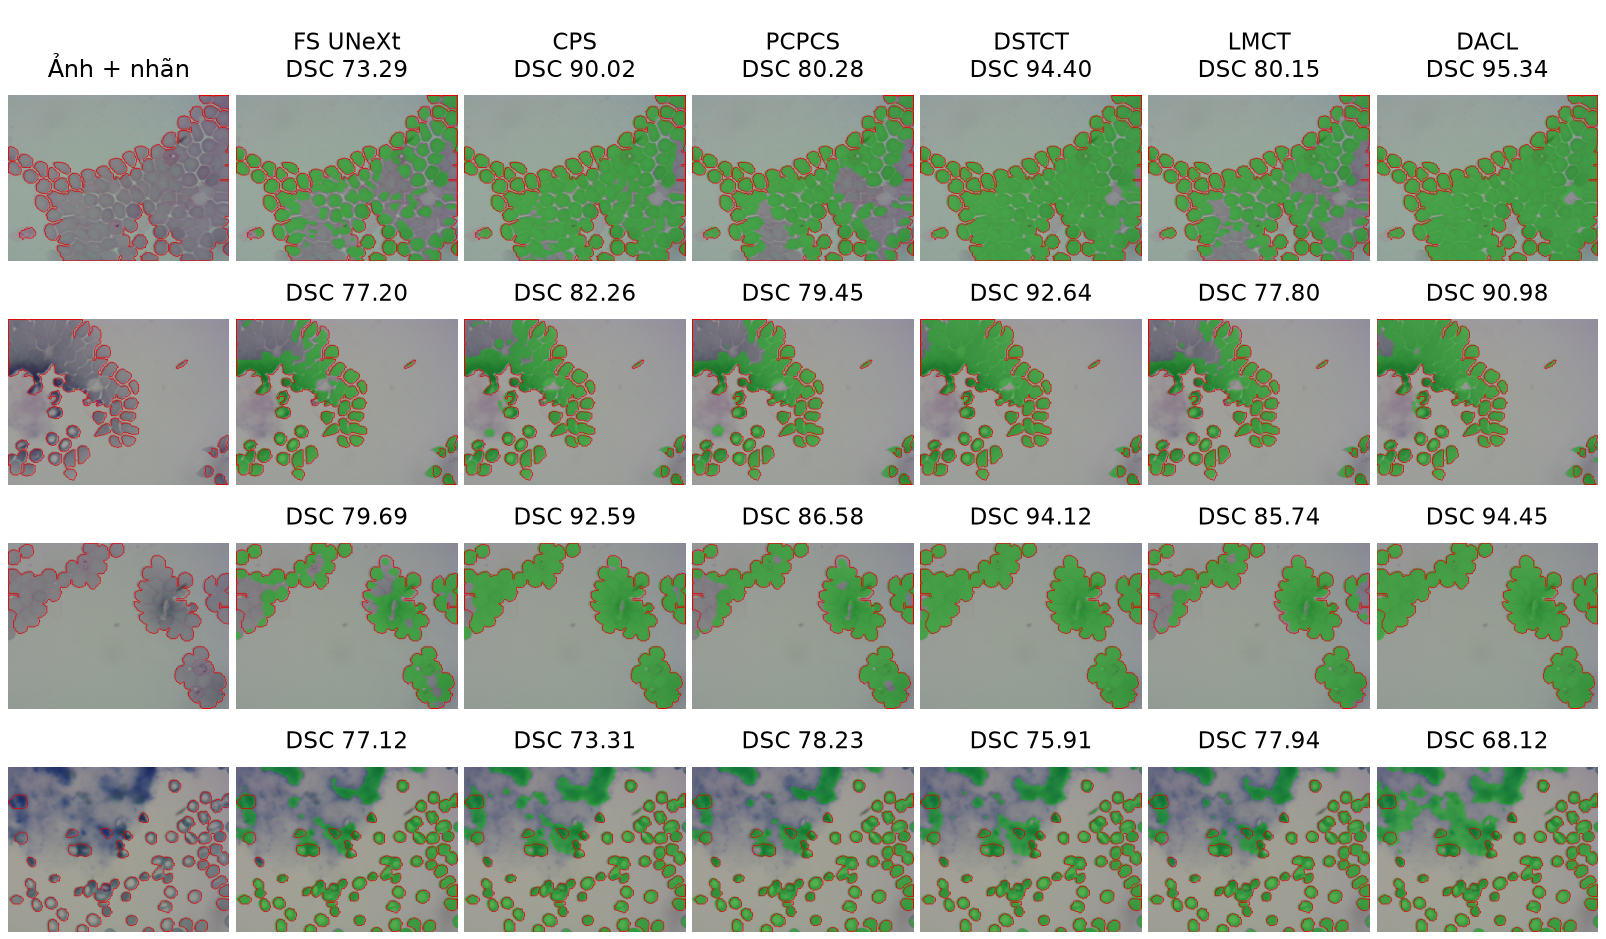
\includegraphics[width=\textwidth]{figures/qualitative_5p.png}
\caption{Kết quả phân đoạn ở mức 5\% nhãn (vùng xanh: dự đoán; viền đỏ: mặt nạ chuẩn; số trên mỗi ô là Dice của ảnh).}
\label{fig:qual}
\end{figure*}

Ở ba ảnh đầu, tế bào xếp thành cụm dày đặc; UNeXt học có giám sát bỏ sót phần lớn bên trong cụm (Dice 73 -- 80\%), trong khi DACL và DSTCT, hai phương pháp có giáo viên EMA của Swin-Unet, phủ gần trọn cụm (trên 90\%). Ở ảnh thứ tư, một mảng cặn nhuộm màu xanh đậm bị mọi mô hình dự đoán nhầm một phần, và DACL nhầm nhiều nhất (68,12\%), phù hợp với HD95 chưa tốt của mô hình. Đây là những trường hợp quan sát được, không đại diện cho toàn bộ tập kiểm thử: bốn ảnh được chọn theo độ phân tán Dice giữa các mô hình, và phân tích ở Bảng~\ref{tab:density} không cho thấy lợi ích tăng theo mật độ tế bào. Các ảnh này chủ yếu minh họa một số trường hợp UNeXt học có giám sát thất bại mà DACL khắc phục được, cùng một kiểu lỗi dương tính giả của DACL.

\begin{figure*}[!t]
\centering
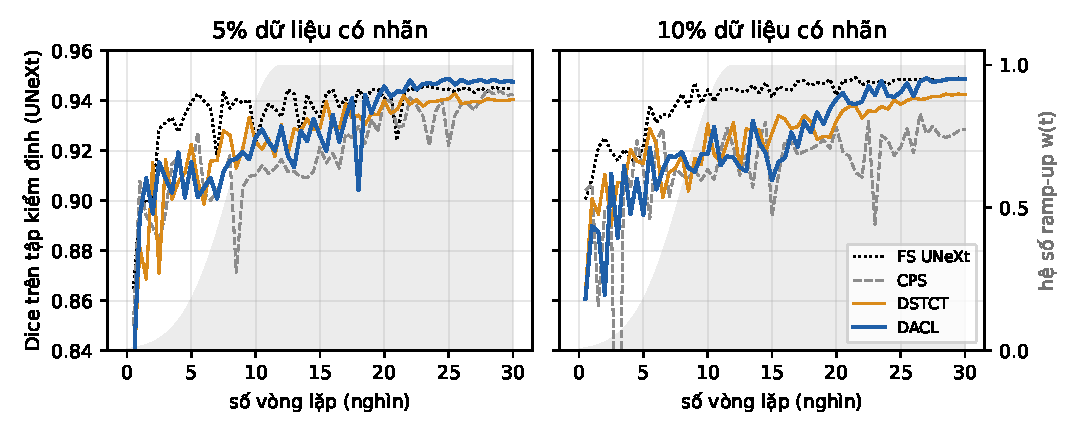
\includegraphics[width=0.85\textwidth]{figures/val_curves.pdf}
\caption{Dice kiểm định của UNeXt theo vòng lặp (vùng xám: hệ số ramp-up).}
\label{fig:curves}
\end{figure*}

Hình~\ref{fig:curves} cho thấy, trong lần huấn luyện này, DACL hội tụ ổn định với bộ trọng số đã chọn. Trong 10.000 vòng cuối ở mức 5\% nhãn, Dice kiểm định của DACL có trung bình 0,9467 và độ lệch chuẩn theo vòng lặp 0,0019, so với 0,9370 và 0,0063 của CPS. Sau giai đoạn ramp-up, phần không giám sát sau khi nhân trọng số chỉ bằng trung bình 18\% phần có giám sát về giá trị mất mát, đúng với mục tiêu đặt ra ở Mục~\ref{sec:weights}; tỷ lệ này không phản ánh trực tiếp mức ảnh hưởng của từng thành phần lên gradient. Hình~\ref{fig:curves} cũng cho thấy UNeXt học có giám sát tăng nhanh hơn các phương pháp bán giám sát ở giai đoạn đầu.

\subsection{Thảo luận}

Kết quả trả lời ba câu hỏi nghiên cứu trong phạm vi một lần huấn luyện cho mỗi cấu hình. Về câu hỏi thứ nhất, DACL dẫn đầu nhóm bán giám sát trên tập kiểm thử nhưng không vượt có ý nghĩa UNeXt học có giám sát trên cùng số nhãn. Việc DSTCT, phương pháp duy nhất khác có giáo viên EMA của Swin-Unet, đứng thứ hai ở mức 10\% gợi ý rằng mục tiêu ổn định từ Swin-Unet tiền huấn luyện có thể là một yếu tố quan trọng; tuy nhiên, vì chỉ nhóm CNN -- Transformer có mạng tiền huấn luyện, khác biệt giữa các nhóm phương pháp không thể quy hoàn toàn cho thuật toán. Về câu hỏi thứ hai, ưu thế của DACL trong nhóm bán giám sát đi kèm precision cao hơn; so với học có giám sát, mức cải thiện lớn chỉ xuất hiện ở một số ảnh mà UNeXt học có giám sát thất bại và không tăng theo mật độ tế bào. Về câu hỏi thứ ba, bộ trọng số \{0,2; 0,2; 1\} đã cho quá trình huấn luyện ổn định trong lần chạy này, điều mà bộ trọng số lớn hơn mười lần không đạt được trong thử nghiệm sơ bộ.

Hai yếu tố có thể giải thích việc DACL chưa vượt học có giám sát, nhưng cả hai đều chưa được kiểm chứng trực tiếp. Thứ nhất, dư địa cải thiện hẹp: 46 ảnh có nhãn đã cho Dice 94,15\%, chỉ kém mức dùng toàn bộ nhãn 1,08 điểm, nên ảnh không nhãn có ít thông tin mới để bổ sung. Thứ hai, mô hình học có giám sát dùng lô 8 ảnh có nhãn, nhận 240.000 lượt ảnh có nhãn trong 30.000 vòng lặp, gấp tám lần các phương pháp bán giám sát. Một đối chứng học có giám sát dùng lô 1 ảnh có nhãn với cùng số bước tối ưu sẽ tách được tác động của số lượt nhìn thấy ảnh có nhãn khỏi tác động của học bán giám sát, nhưng chưa được thực hiện. So sánh giữa các phương pháp bán giám sát với nhau không chịu ảnh hưởng này vì chúng dùng chung cách bố trí lô. HD95 chưa tốt có thể liên quan đến thành phần cực tiểu hóa entropy trong $\Lx{dac}$: dự đoán sai nhưng tự tin trên vùng cặn nhuộm tạo thành một vùng dương tính giả trọn vẹn; giả thuyết này cần được kiểm chứng bằng thí nghiệm loại bỏ $\Lx{ent}$.

Về giá trị ứng dụng, với 46 ảnh có nhãn, UNeXt huấn luyện bằng DACL đạt Dice 94,38\%, chỉ kém Swin-Unet học có giám sát 0,34 điểm trong khi cần 1,80 GFLOPs so với 12,15 GFLOPs, phù hợp cho triển khai trên thiết bị có tài nguyên hạn chế. Cần lưu ý rằng chính UNeXt học có giám sát trên cùng 46 ảnh đã đạt 94,15\%, nên giá trị ứng dụng này chủ yếu đến từ bản thân mạng nhẹ; phần đóng góp thêm của DACL trên bộ dữ liệu này nhỏ và chưa có ý nghĩa thống kê.

Nghiên cứu còn các giới hạn sau. Mỗi cấu hình chỉ được huấn luyện một lần với hạt giống 2026 và một cách chọn ảnh có nhãn, trong khi dao động giữa các lần huấn luyện có thể gần một điểm Dice, nên các kết luận thống kê chỉ áp dụng cho các mô hình cụ thể đã huấn luyện. Chưa có thí nghiệm lặp với nhiều hạt giống, thí nghiệm loại bỏ từng thành phần mất mát, đối chứng học có giám sát cùng bố trí lô, khảo sát trọng số hay đo chuẩn gradient. Các phương pháp đối chứng dùng trọng số mặc định, một số được điều chỉnh so với bản gốc, và chỉ nhóm CNN -- Transformer có mạng tiền huấn luyện. Ảnh được xử lý ở 224$\times$224 nên một phần khe tách giữa tế bào bị mất. Cuối cùng, bộ dữ liệu không có mã tiêu bản hay mã người bệnh, nên tính độc lập giữa các tập mới chỉ được kiểm tra ở mức ảnh trùng hoặc gần trùng.

% ======================================================================
\section{Kết luận}
\label{sec:conclusion}

Đây là một nghiên cứu thực nghiệm và phân tích ứng dụng về khung học bán giám sát DACL cho bài toán phân đoạn tế bào máu trong ảnh hiển vi khi dữ liệu có nhãn khan hiếm. Kiến trúc và các hàm mất mát được kế thừa từ DACL; phần việc của nhóm tác giả là chuyển khung sang miền ảnh hiển vi, tái triển khai nó cùng tám phương pháp đối chứng trong một giao thức thống nhất, phân tích số hạng entropy để lựa chọn trọng số, và phân tích sai số theo loại lỗi, độ khó và mật độ tế bào.

Trên bộ dữ liệu Blood Cell Segmentation, UNeXt 1,58 triệu tham số huấn luyện bằng DACL đạt Dice 94,38\% và 94,46\% ở mức 5\% và 10\% nhãn, cao nhất trong chín phương pháp bán giám sát được cài đặt lại; khác biệt có ý nghĩa theo kiểm định Wilcoxon trên ảnh kiểm thử, cho các mô hình đã huấn luyện một lần. Tuy nhiên, so với UNeXt học có giám sát trên cùng số nhãn, DACL chỉ cao hơn 0,23 điểm ở mức 5\% (không có ý nghĩa thống kê) và thấp hơn 0,14 điểm ở mức 10\%, nên nghiên cứu không kết luận rằng DACL cải thiện so với học có giám sát trên bộ dữ liệu này. Phân tích theo mật độ tế bào không cho thấy lợi ích tăng theo mật độ; mức cải thiện lớn chỉ quan sát được ở một số ảnh mà mô hình học có giám sát thất bại. Về mặt phương pháp, phân tích hàm đồng thuận kép cho thấy số hạng entropy trở thành cực tiểu hóa entropy khi hai mạng đồng thuận, và cùng với độ lớn giá trị các thành phần mất mát, cung cấp căn cứ để chọn bộ trọng số \{0,2; 0,2; 1\}. Vì mạng nhẹ đạt độ chính xác gần Swin-Unet, kết quả có thể làm cơ sở cho các hệ thống hỗ trợ đếm và đo tế bào tại phòng xét nghiệm có ít dữ liệu gán nhãn.

Mô hình chưa cải thiện HD95, một phần do các dự đoán nhầm trên vùng cặn nhuộm. Trong giai đoạn tiếp theo, các thí nghiệm chính sẽ được lặp lại với ít nhất ba hạt giống và các cách chọn ảnh có nhãn khác nhau, kèm đối chứng học có giám sát dùng cùng bố trí lô, để đánh giá độ ổn định của thứ hạng. Nghiên cứu cũng dự kiến thực hiện thí nghiệm loại bỏ từng thành phần mất mát, đặc biệt là $\Lx{ent}$, đo chuẩn gradient của từng thành phần và khảo sát có hệ thống ảnh hưởng của trọng số. Bên cạnh đó, việc huấn luyện ở độ phân giải cao hơn sẽ giúp giữ lại khe tách giữa các tế bào chạm nhau, và bước tách, đếm từng tế bào sẽ được bổ sung để đánh giá mô hình trên chính tác vụ ứng dụng.

% ======================================================================
\begin{thebibliography}{00}
\bibitem{unet} O. Ronneberger, P. Fischer, and T. Brox, ``U-Net: Convolutional networks for biomedical image segmentation,'' in \textit{Proc. MICCAI}, 2015, pp. 234--241.
\bibitem{depto} D. S. Depto, S. Rahman, M. M. Hosen, \textit{et al.}, ``Automatic segmentation of blood cells from microscopic slides: A comparative analysis,'' \textit{Tissue and Cell}, vol. 73, p. 101653, 2021.
\bibitem{survey} J. E. van Engelen and H. H. Hoos, ``A survey on semi-supervised learning,'' \textit{Machine Learning}, vol. 109, no. 2, pp. 373--440, 2020.
\bibitem{confirm} E. Arazo, D. Ortego, P. Albert, N. E. O'Connor, and K. McGuinness, ``Pseudo-labeling and confirmation bias in deep semi-supervised learning,'' in \textit{Proc. IJCNN}, 2020, pp. 1--8.
\bibitem{dacl} F. Wang, G. Silvestre, Z. Wang, and K. M. Curran, ``Dual agreement consistency learning for semi-supervised fetal ultrasound segmentation,'' \textit{arXiv preprint} arXiv:2606.25254, 2026.
\bibitem{repo} D. S. Depto \textit{et al.}, ``Blood-cell-segmentation,'' GitHub repository, 2021. [Online]. Available: \url{https://github.com/Deponker/Blood-cell-segmentation}
\bibitem{hed} D. Tellez, M. Balkenhol, I. Otte-H\"{o}ller, \textit{et al.}, ``Whole-slide mitosis detection in H\&E breast histology using PHH3 as a reference to train distilled stain-invariant convolutional networks,'' \textit{IEEE Transactions on Medical Imaging}, vol. 37, no. 9, pp. 2126--2136, 2018.
\bibitem{unext} J. M. J. Valanarasu and V. M. Patel, ``UNeXt: MLP-based rapid medical image segmentation network,'' in \textit{Proc. MICCAI}, 2022, pp. 23--33.
\bibitem{swinunet} H. Cao, Y. Wang, J. Chen, \textit{et al.}, ``Swin-Unet: Unet-like pure Transformer for medical image segmentation,'' in \textit{Proc. ECCV Workshops}, 2022, pp. 205--218.
\bibitem{swin} Z. Liu, Y. Lin, Y. Cao, \textit{et al.}, ``Swin Transformer: Hierarchical vision Transformer using shifted windows,'' in \textit{Proc. ICCV}, 2021, pp. 10012--10022.
\bibitem{imagenet} J. Deng, W. Dong, R. Socher, \textit{et al.}, ``ImageNet: A large-scale hierarchical image database,'' in \textit{Proc. CVPR}, 2009, pp. 248--255.
\bibitem{dice} F. Milletari, N. Navab, and S.-A. Ahmadi, ``V-Net: Fully convolutional neural networks for volumetric medical image segmentation,'' in \textit{Proc. 3DV}, 2016, pp. 565--571.
\bibitem{dct} S. Qiao, W. Shen, Z. Zhang, B. Wang, and A. Yuille, ``Deep co-training for semi-supervised image recognition,'' in \textit{Proc. ECCV}, 2018, pp. 135--152.
\bibitem{cps} X. Chen, Y. Yuan, G. Zeng, and J. Wang, ``Semi-supervised semantic segmentation with cross pseudo supervision,'' in \textit{Proc. CVPR}, 2021, pp. 2613--2622.
\bibitem{ctct} X. Luo, M. Hu, T. Song, G. Wang, and S. Zhang, ``Semi-supervised medical image segmentation via cross teaching between CNN and Transformer,'' in \textit{Proc. MIDL}, 2022, pp. 820--833.
\bibitem{ict} V. Verma, K. Kawaguchi, A. Lamb, \textit{et al.}, ``Interpolation consistency training for semi-supervised learning,'' \textit{Neural Networks}, vol. 145, pp. 90--106, 2022.
\bibitem{mixup} H. Zhang, M. Cisse, Y. N. Dauphin, and D. Lopez-Paz, ``mixup: Beyond empirical risk minimization,'' in \textit{Proc. ICLR}, 2018.
\bibitem{mt} A. Tarvainen and H. Valpola, ``Mean teachers are better role models: Weight-averaged consistency targets improve semi-supervised deep learning results,'' in \textit{Proc. NeurIPS}, 2017.
\bibitem{kl} S. Kullback and R. A. Leibler, ``On information and sufficiency,'' \textit{The Annals of Mathematical Statistics}, vol. 22, no. 1, pp. 79--86, 1951.
\bibitem{rampup} S. Laine and T. Aila, ``Temporal ensembling for semi-supervised learning,'' in \textit{Proc. ICLR}, 2017.
\bibitem{jsd} J. Lin, ``Divergence measures based on the Shannon entropy,'' \textit{IEEE Transactions on Information Theory}, vol. 37, no. 1, pp. 145--151, 1991.
\bibitem{entmin} Y. Grandvalet and Y. Bengio, ``Semi-supervised learning by entropy minimization,'' in \textit{Advances in Neural Information Processing Systems 17}, 2005, pp. 529--536.
\bibitem{ssl4mis} X. Luo, ``SSL4MIS: Semi-supervised learning for medical image segmentation,'' GitHub repository, 2020. [Online]. Available: \url{https://github.com/HiLab-git/SSL4MIS}
\bibitem{poly} L.-C. Chen, G. Papandreou, I. Kokkinos, K. Murphy, and A. L. Yuille, ``DeepLab: Semantic image segmentation with deep convolutional nets, atrous convolution, and fully connected CRFs,'' \textit{IEEE Transactions on Pattern Analysis and Machine Intelligence}, vol. 40, no. 4, pp. 834--848, 2018.
\bibitem{pcpcs} C. Ma and Z. Wang, ``Semi-Mamba-UNet: Pixel-level contrastive and cross-supervised visual Mamba-based UNet for semi-supervised medical image segmentation,'' \textit{Knowledge-Based Systems}, vol. 300, p. 112203, 2024.
\bibitem{dstct} J. Jiang, H. Wang, J. Bai, \textit{et al.}, ``Intrapartum ultrasound image segmentation of pubic symphysis and fetal head using dual student-teacher framework with CNN-ViT collaborative learning,'' in \textit{Proc. MICCAI}, 2024, pp. 448--458.
\bibitem{lmct} F. Wang, K. M. Curran, and G. Silvestre, ``Semi-supervised cervical segmentation on ultrasound by a dual framework for neural networks,'' in \textit{Proc. IEEE ISBI}, 2025.
\bibitem{metrics} A. A. Taha and A. Hanbury, ``Metrics for evaluating 3D medical image segmentation: Analysis, selection, and tool,'' \textit{BMC Medical Imaging}, vol. 15, p. 29, 2015.
\bibitem{wilcoxon} F. Wilcoxon, ``Individual comparisons by ranking methods,'' \textit{Biometrics Bulletin}, vol. 1, no. 6, pp. 80--83, 1945.
\bibitem{bonferroni} O. J. Dunn, ``Multiple comparisons among means,'' \textit{Journal of the American Statistical Association}, vol. 56, no. 293, pp. 52--64, 1961.
\end{thebibliography}

\end{document}
